\renewcommand{\baselinestretch}{1.5}
\fontsize{12pt}{13pt}\selectfont

\chapter{实验与评估} \label{experiment}

在第四章仿真中,已经完成单机控制和多机控制的实验,并且完成了单机SLAM和双机协同SLAM的仿真实验。但是为了实验的完整性,必须使用实际场景中获得的视频进行实验,
这包括数据集、录像视频转rosbag、T265相机实时视频等方式的实验。
实验内容主要有两部分,单机的SLAM实验和多机的SLAM实验。

\section{Euroc数据集实验}

Euroc数据集是苏黎世联邦理工大学制作,本实验使用其中两个“简单”类型的数据集。该数据集使用配备双目相机和IMU的小型无人机录制。虽然是可以直接获取深度的双目相机,但本研究选取的两个数据集在开始时,均进行了多次上下和左右平移运动,可以满足单目相机初始化的任务,因此该数据集完全可以用于单目SLAM的实验\footnote{https://projects.asl.ethz.ch/datasets/doku.php?id=kmavvisualinertialdatasets}。

为了做更加精确的比较,数据集除了rosbag或图片序列之外,还需要位姿真值信息,用于比对定位的精度;此外,还需要时间戳信息,因为SLAM系统记录下来的是关键帧的位姿及时间戳,但关键帧的数量远远小于整个视频的帧数,因此需要通过时间戳的匹配来分析当前关键帧的位姿。

\begin{figure}[htbp]
	\centering
	\begin{minipage}[t]{0.45\columnwidth} %小于1/n如果使用n张图片
		\centering
		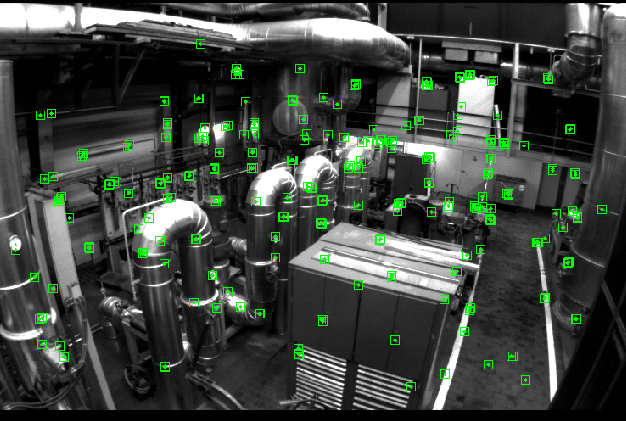
\includegraphics[width=1.0\columnwidth]{euroc1.png}
		\caption{无人机1当前帧}
		\label{fig-euroc1}
	\end{minipage}
	\begin{minipage}[t]{0.45\columnwidth}
		\centering
		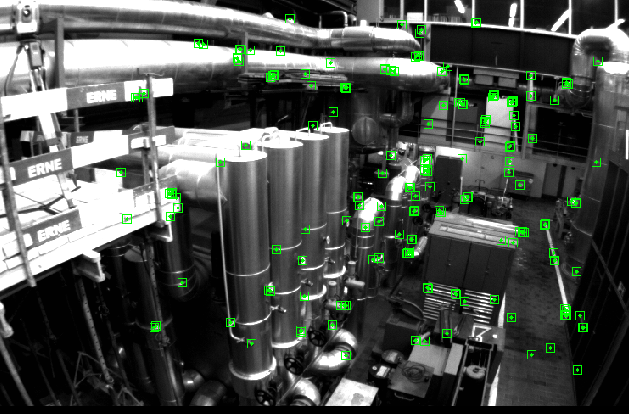
\includegraphics[width=1.0\columnwidth]{euroc2.png}
		\caption{无人机2当前帧}
		\label{fig-euroc2}
	\end{minipage}
\end{figure}

图\ref{fig-euroc1},\ref{fig-euroc2}展示了两架无人机在飞行过程中ORB-SLAM2当前帧的画面,该场景是ETH一个工业实验室内部的场景,使用微型无人机可以很容易地在该环境中穿梭,完成较好的定位与建图任务。

图\ref{fig-euroc3}展示了两架无人机各自的地图,图像右侧展示了两机拼合的地图;图\ref{fig-euroc4}为方法后的地图拼合场景,可以看到地图拼合之后,两者的出发点也被合并到同一位置,这与实际情况相符,接下来需要使用轨迹工具来验证两者的实际轨迹是否与建图相符。

\begin{figure}[htbp]
	\centering
	\begin{minipage}[t]{0.45\columnwidth} %小于1/n如果使用n张图片
		\centering
		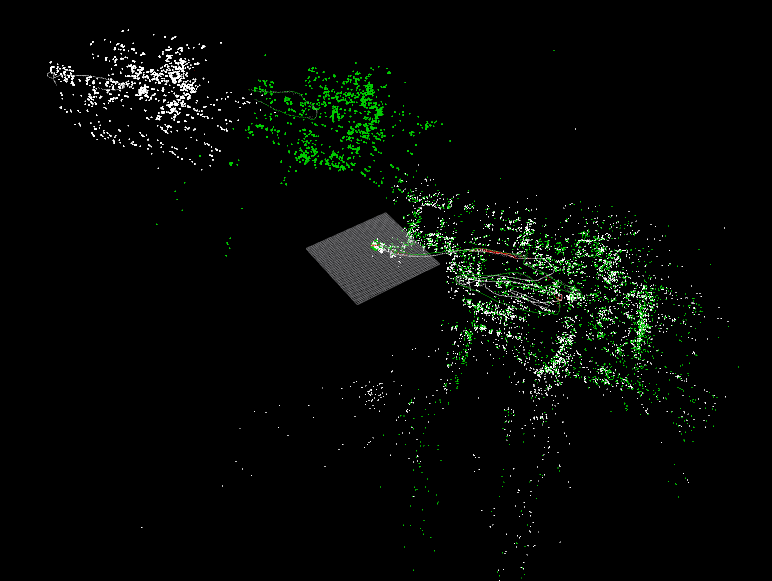
\includegraphics[width=1.0\columnwidth]{euroc3.png}
		\caption{双机地图和拼合地图}
		\label{fig-euroc3}
	\end{minipage}
	\begin{minipage}[t]{0.45\columnwidth}
		\centering
		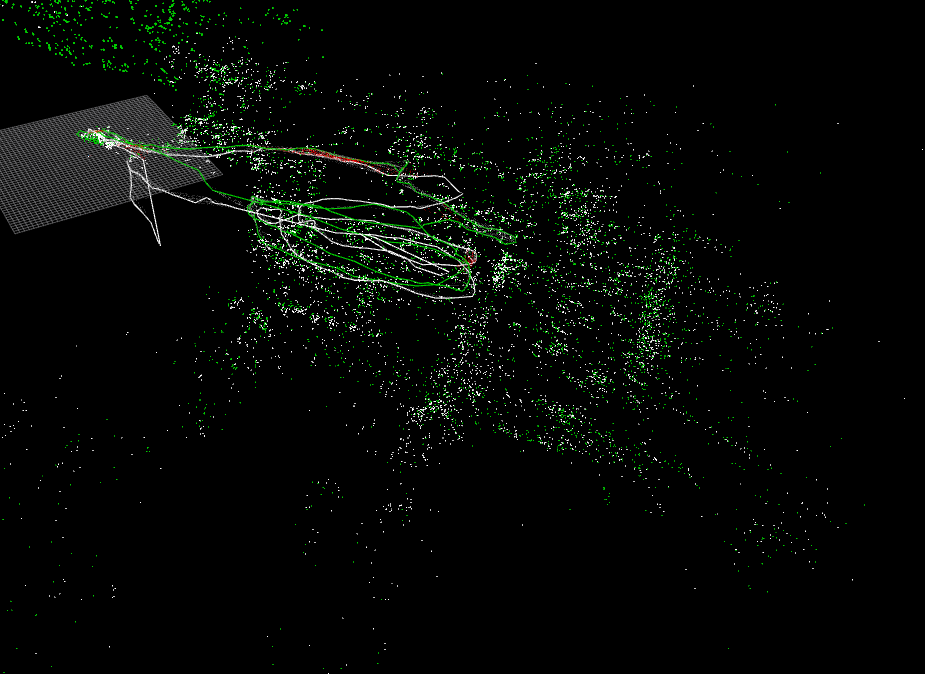
\includegraphics[width=1.0\columnwidth]{euroc4.png}
		\caption{双机轨迹和拼合地图}
		\label{fig-euroc4}
	\end{minipage}
\end{figure}

evo是由Michael Grupp开发的一款专门针对SLAM的轨迹可视化与位姿分析软件,其支持TUM、Euroc、KITTI的数据集格式,并且可以相互转换;支持位姿真值轨迹与SLAM得到的轨迹进行Sim3转化,得到对齐之后的位姿真值与视觉轨迹比较;并且可以分析绝对误差,评判算法的准确性\footnote[1]{https://github.com/MichaelGrupp/evo/wiki}。

\begin{figure}[htbp]
	\centering
	\begin{minipage}[t]{0.45\columnwidth} %小于1/n如果使用n张图片
		\centering
		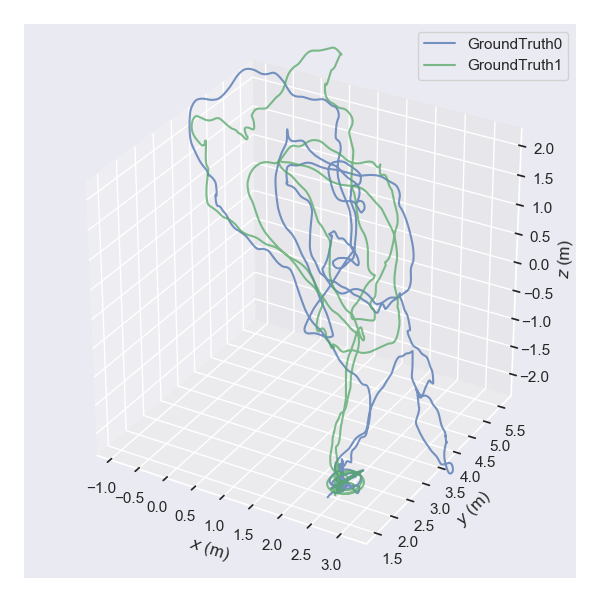
\includegraphics[width=1.0\columnwidth]{groundtruth.png}
		\caption{双机位姿真值}
		\label{fig-groundtruth}
	\end{minipage}
	\begin{minipage}[t]{0.45\columnwidth}
		\centering
		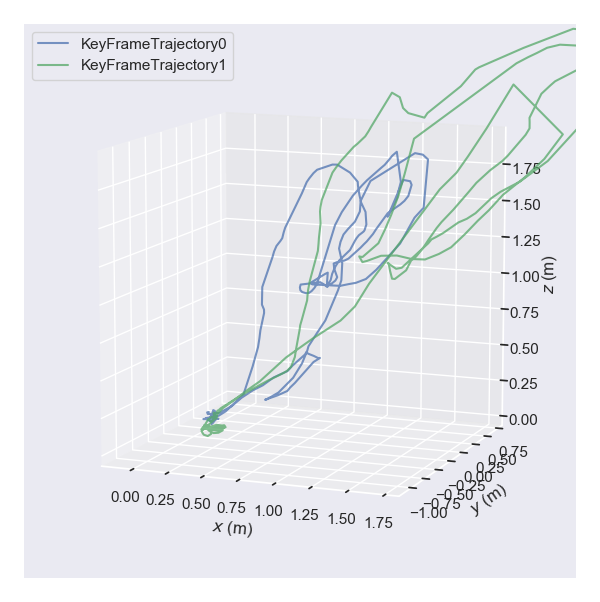
\includegraphics[width=1.0\columnwidth]{trajectory.png}
		\caption{双机位姿估计}
		\label{fig-trajectory}
	\end{minipage}
\end{figure}

图\ref{fig-groundtruth}展示了数据集提供的两架无人机的位姿真值,该真值由红外运动捕捉相机测量得到。图\ref{fig-trajectory}展示了两架无人机通过SLAM方法得到的轨迹估计,由于轨迹估计在坐标系和尺度上与实际真值存在一定转换关系,只从这两幅图像中无法得到对于单架无人机而言,位姿估计和真值的关系,因此需要使用evo自带的Sim3转换,得到校正过的真值与估计的拼合图像。

\begin{figure}[htbp]
	\centering
	\begin{minipage}[t]{0.45\columnwidth} %小于1/n如果使用n张图片
		\centering
		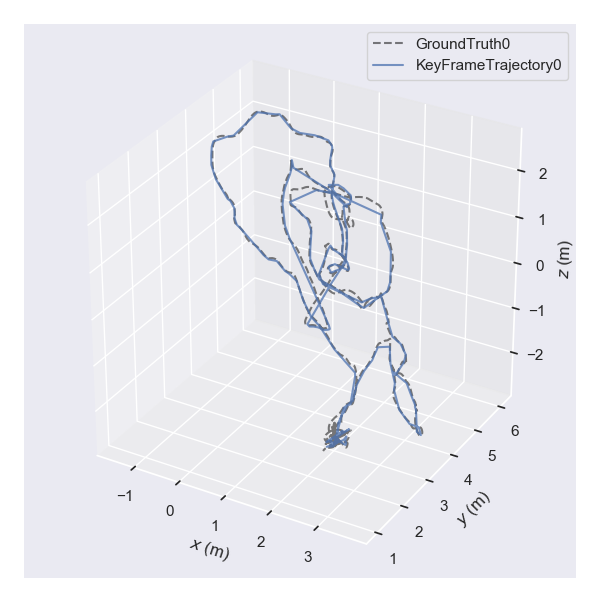
\includegraphics[width=1.0\columnwidth]{comp0.png}
		\caption{无人机0真值与估计对比}
		\label{fig-comp0}
	\end{minipage}
	\begin{minipage}[t]{0.45\columnwidth}
		\centering
		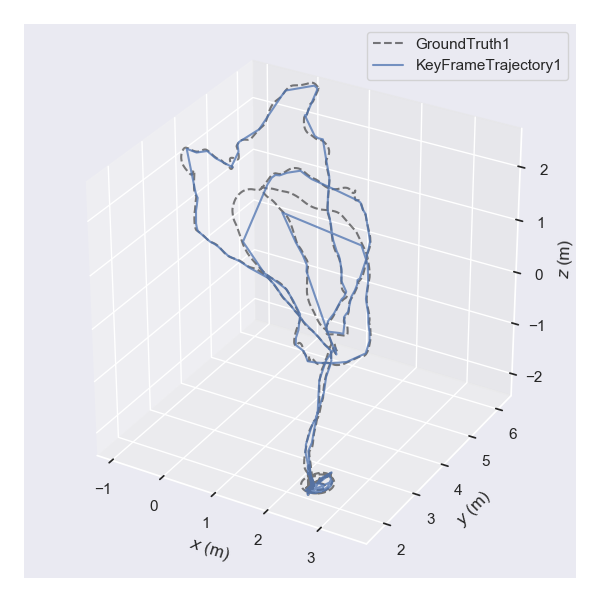
\includegraphics[width=1.0\columnwidth]{comp1.png}
		\caption{无人机1真值与估计对比}
		\label{fig-comp1}
	\end{minipage}
\end{figure}

在图\ref{fig-comp0},\ref{fig-comp1}中,虚线均代表各自的位姿真值,实线均代表各自的位姿估计值,可以看出整体上视觉位姿估计的效果较好,与真值的误差较小,但是仍需要通过进一步的计算和比对来确定误差。evo提供了计算绝对误差的工具。

\begin{figure}[htbp]
	\centering
	\begin{minipage}[t]{0.45\columnwidth} %小于1/n如果使用n张图片
		\centering
		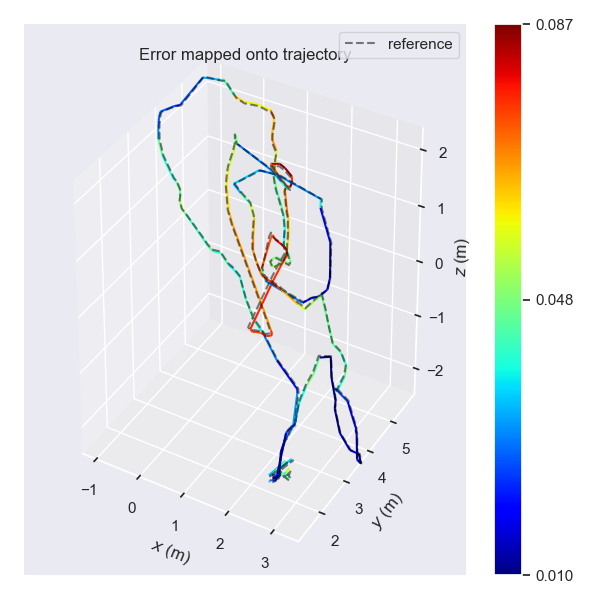
\includegraphics[width=1.0\columnwidth]{ape_map0.png}
		\caption{无人机0轨迹误差}
		\label{fig-apemap0}
	\end{minipage}
	\begin{minipage}[t]{0.45\columnwidth}
		\centering
		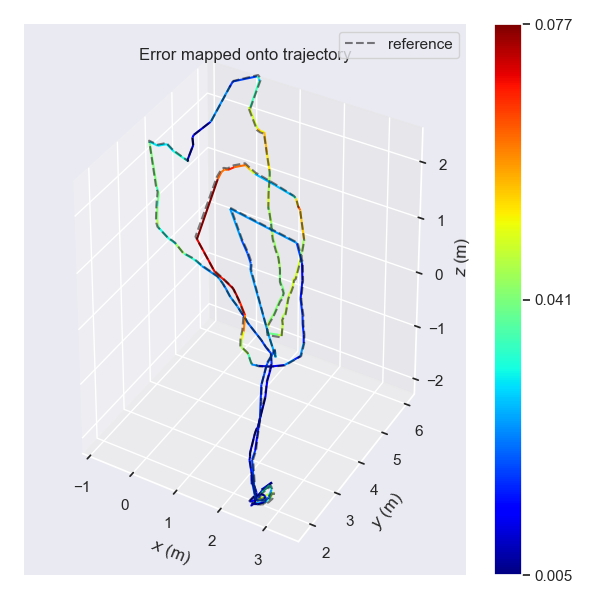
\includegraphics[width=1.0\columnwidth]{ape_map1.png}
		\caption{无人机1轨迹误差}
		\label{fig-apemap1}
	\end{minipage}
\end{figure}

图\ref{fig-apemap0},\ref{fig-apemap1}表现了两机整个飞行轨迹中的误差变化,颜色越暖则误差越大,颜色越冷则误差越小。通过对照图分析可以发现,在轨迹变化不光滑的区域,颜色为红色,误差最大,这与实际情况是相符的,往往是经过了重定位或经历了短暂的跟踪丢失的情况。但是这样的描述仍然不具有说服力,于是本文采用了更为直观的表示方法。

\begin{figure}[!ht]
	\centering
	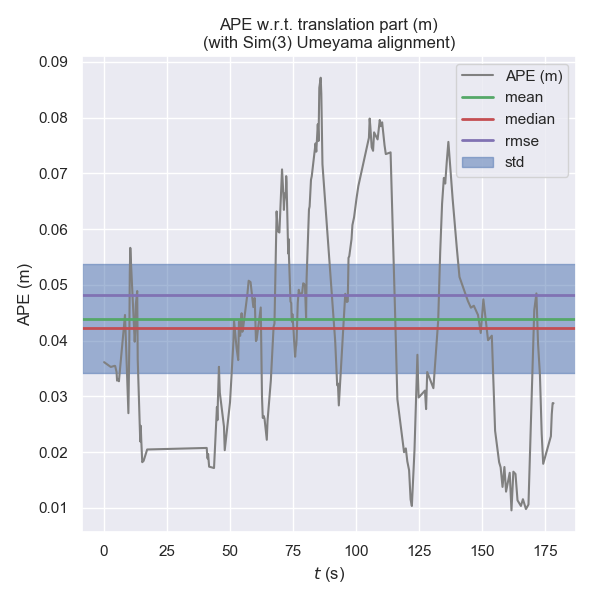
\includegraphics[width=0.7\textwidth]{ape_raw0.png}
	\caption{无人机0误差分析}
	\label{fig-aperaw0}
\end{figure}

图\ref{fig-aperaw0}展示了无人机0的整体轨迹估计误差分析图,图中包含了其最大误差和均值、中间值等参数,可以看出相对于以真值为维度的参考下,结合图\ref{fig-apemap0}中所示的颜色误差分析和表\ref{error-euroc}中的各参数具体值可以给出结论,视觉SLAM的误差满足定位精度要求。

\begin{table}[!htbp]
	\centering
	\caption{无人机0误差表}\label{error-euroc}%添加标题 设置标签
	\begin{tabular}{ccccccc}
		\toprule
		
		max& mean & median & min & rmse & sse & std\\
		0.087 & 0.044 & 0.042 &  0.010 & 0.048 & 0.475 & 0.020\\
		
		\bottomrule
	\end{tabular}
\end{table}

\section{单机SLAM实验}

真机搭载英特尔T265摄像头,其特点是带两个鱼眼镜头和惯性测量单元,并且视觉SLAM可以运行在其特有的视觉处理单元上。其在电脑上需要一定配置,安装英特尔的一些依赖库文件和realsense-viewer。

除摄像头外,真机还搭载Jetson Xavier NX计算机,体积较小且接口丰富。需要注意的是,无人机在地面时,可以使用显示器和鼠标设备对其进行操作,运行ROS节点;但当无人机在空中时,没有显示信息和鼠标的操作输入,因此需要使用远程控制,在这里使用了No Machine软件进行远程控制。

实验内容如下:

在真机实验之前,首先使用T265相机中的单目相机进行室内的建图实验;使用单目相机进行ORB-SLAM2的关键是初始化,这是由单目相机的特性决定的;由于其拍摄到的图片不具有深度信息,因此需要依靠三角化恢复深度。而三角化的特点是,两帧之间的平移向量不能为零,否则解出的旋转矩阵也为零;因此单目相机的初始化方法是使相机在相同场景中不断左右或上下平移。初始化成功后,ORB-SLAM2进入跟踪模式,需要注意当进入陌生场景(比如直角转弯)时,移动应尽量缓慢,否则很容易跟丢,进入重定位模式。
但进入重定位模式后,只要将视角对准经历过的场景,一般又能重新恢复跟踪。

共进行两个场景的稀疏点云建图,如图\ref{result1},图\ref{result2}所示:

\begin{figure}[htbp]
	\centering
	\begin{minipage}[t]{0.45\columnwidth} %小于1/n如果使用n张图片
		\centering
		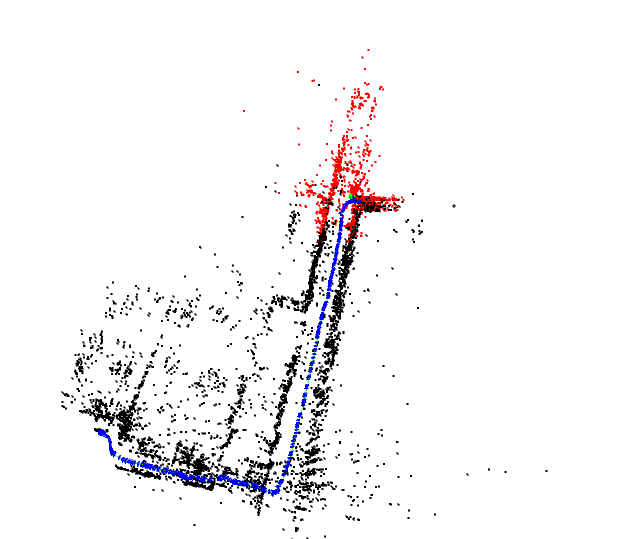
\includegraphics[width=1.0\columnwidth]{ou1-1.png}
		\caption{教东B一楼楼道}
		\label{result1}
	\end{minipage}
	\begin{minipage}[t]{0.45\columnwidth}
		\centering
		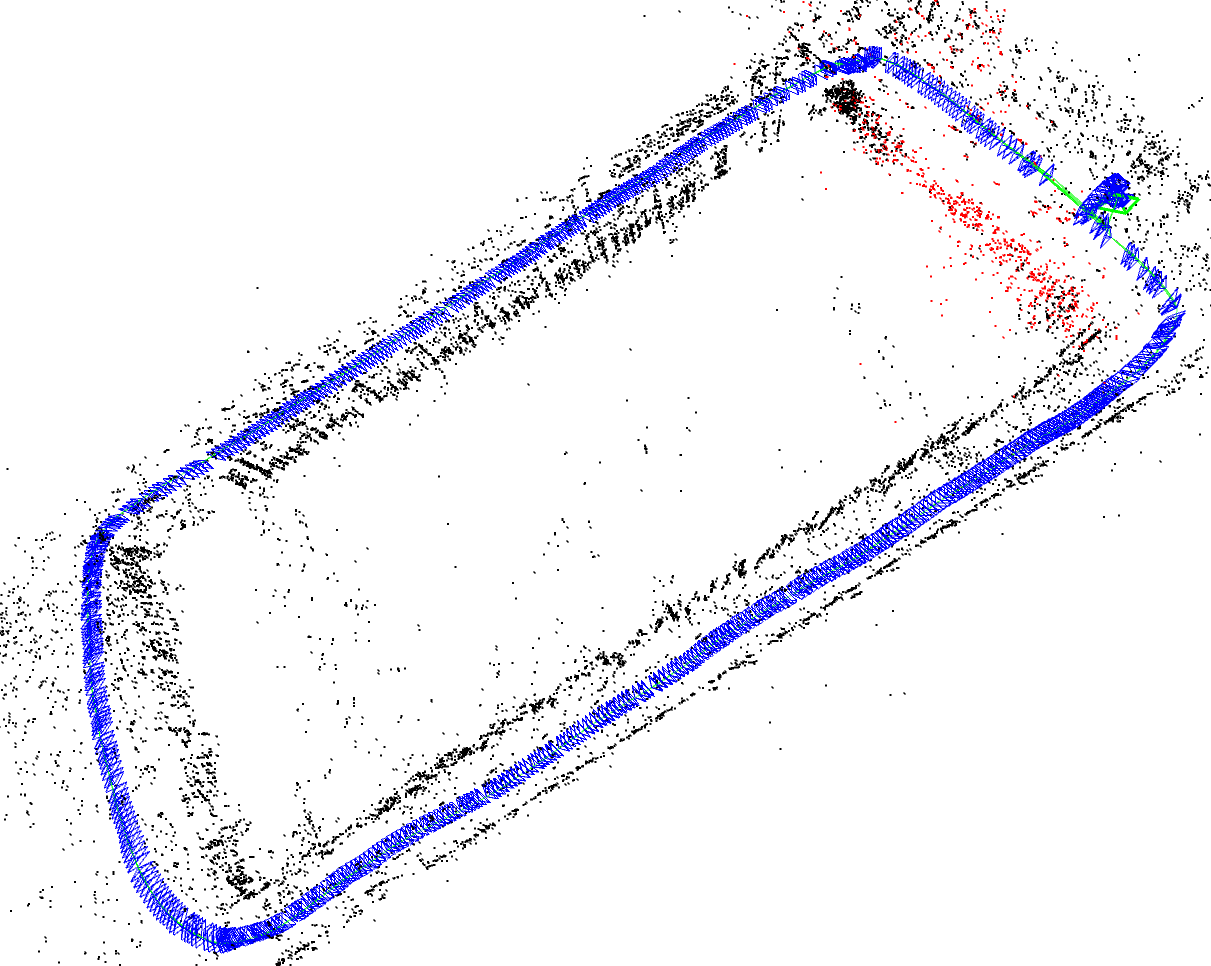
\includegraphics[width=1.0\columnwidth]{ou3-1.png}
		\caption{教东C二楼楼道}
		\label{result2}
	\end{minipage}
\end{figure}


\section{多机SLAM实验}

由于多机SLAM实验需要一定的场景和操作人员,编队飞行进行SLAM过程中的的安全性无法保证,因此只进行了简单的多机起降实验,具体的多机SLAM实验采用相机录制视频转rosbag的形式进行。

在教学楼楼道场景下,使用手持相机的方式,沿楼道行走,完成对一段楼道的建图;同时准备另一台相机,沿不同的路线行进,完成对同一段楼道的建图;两段视频应该拥有一部分重合的场景和一部分不重合的场景,用以验证地图融合的效果。

需要注意的是,使用单目视觉SLAM时,初始化是一个重要的步骤,一般采用在一个场景左右平移的方法完成初始化,之后才能进行跟踪进程,否则一段视频中将会有大量的时间用于初始化,这也意味着选取视频的质量十分重要。

在进行SLAM进程前,需要对相机进行标定,可以采用张正友标定法;需要注意的是,相机的拍照模式和录像模式,其内参矩阵可能不同;对于使用视觉SLAM的相机,建议采用动态标定法。

最后,使用预先录制的视频验证SLAM算法有两个方式:

\begin{enumerate}
	\item 将视频转换成KITTI或TUM数据集的格式;通过观察这些数
	据集的格式可以看出,其一般是灰度图加深度信息,并且配有时间戳,这样的转换可能有一些复杂。转换完成后,使用ROS的例子中自带的对于特定传感器和特定数据集的可执行文件运行整个SLAM进程即可。
	\item 较为简单的方式是将其转换为ROS的rosbag,rosbag可以记录特定话题的信息;对于视频而言,即记录不同时间戳下矩阵各点的三通道RGB值,对于灰度视频则更为方便;其用法是使用ROS的cv bridge完成一些MP4格式视频到rosbag包的转换。
\end{enumerate}

完成MP4格式到rosbag转换,
其主要逻辑是,将每一帧的信息转换成sensor\_msg类型的消息,之后写入到rosbag中。这里需要注意waitKey函数,其含义为循环等待,单位是1/1000秒,因此1000/fps即为按照fps帧率,每一帧需要等待的时间;该参数控制了视频的帧率,从而控制了rosbag包的长度。topicName为录制的话题名,已经提前定义好。

实验在教东B教室进行,从后门和窗户两个方向相向而行,录制两段视频,尽量保证两段视频中出现重叠场景,以方便地图融合;

\begin{figure}[htbp]
	\centering
	\begin{minipage}[t]{0.45\columnwidth} %小于1/n如果使用n张图片
		\centering
		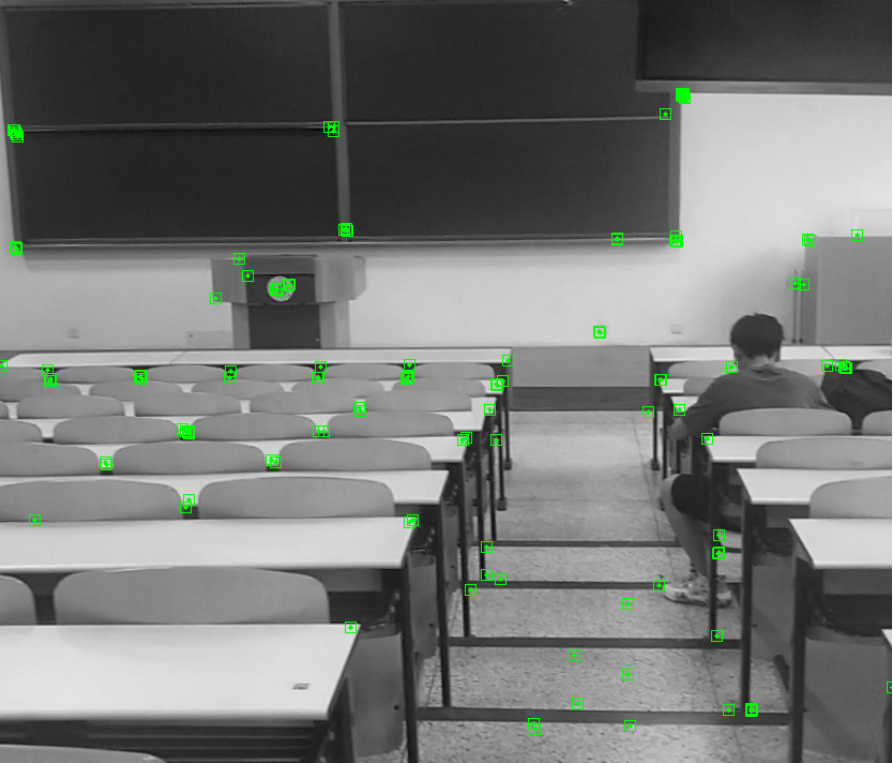
\includegraphics[width=1.0\columnwidth]{ccm4.png}
		\caption{教室特征点匹配示例}
		\label{fig5-1}
	\end{minipage}
	\begin{minipage}[t]{0.45\columnwidth}
		\centering
		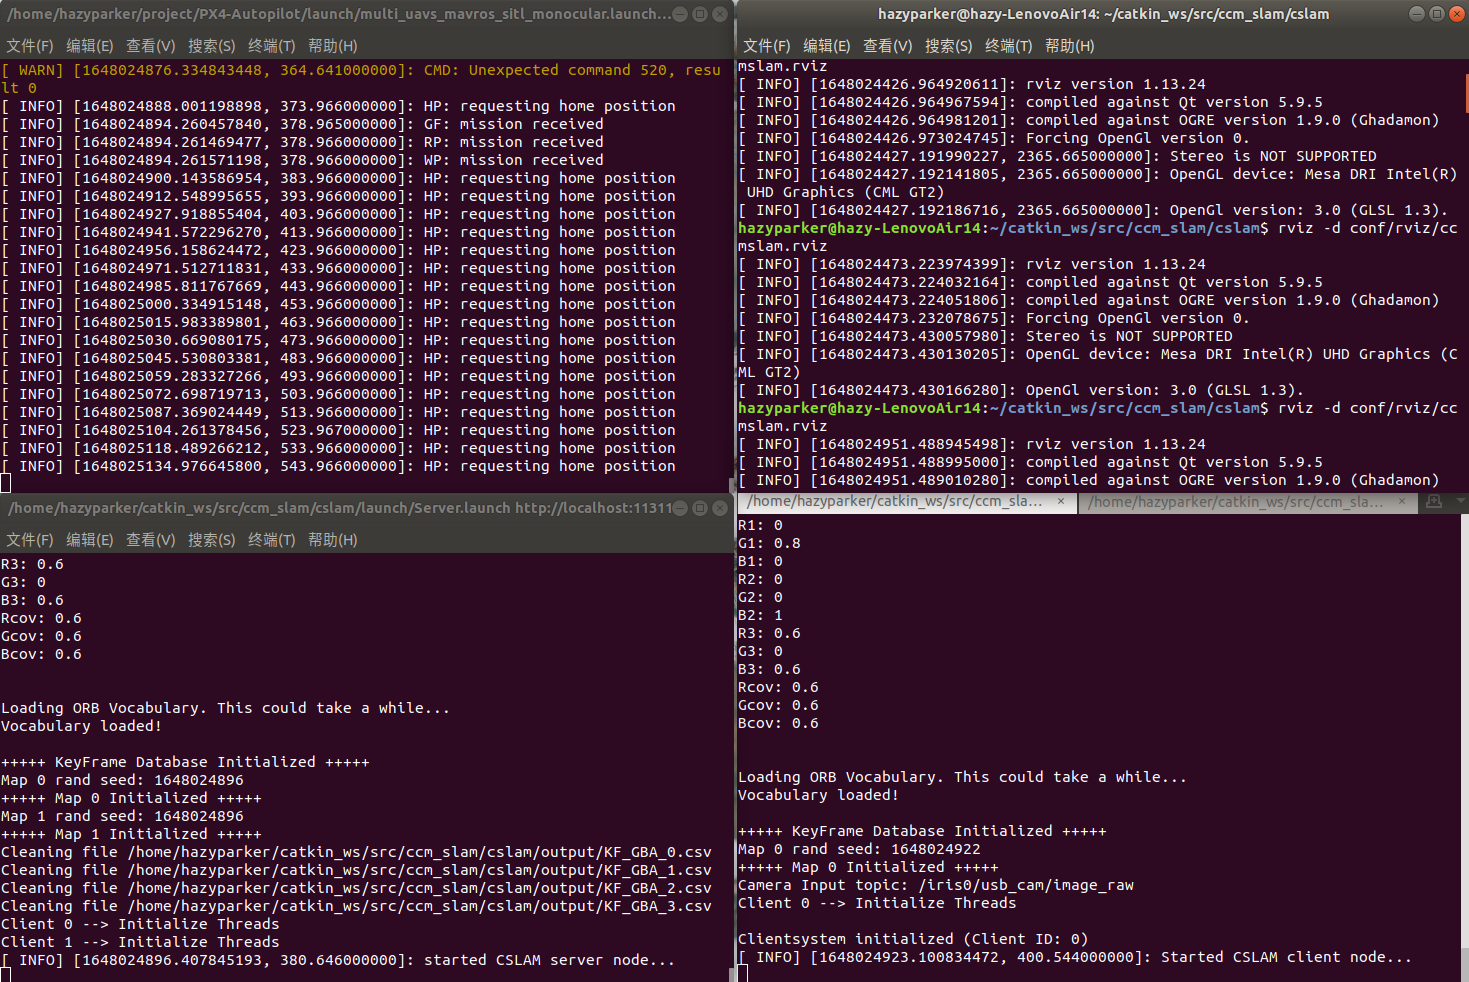
\includegraphics[width=1.0\columnwidth]{ccm2.png}
		\caption{地图融合}
		\label{fig5-2}
	\end{minipage}
\end{figure}

可以看出,基本完成了建图和地图融合的任务。